%!TEX program = xelatex

\documentclass[11pt,titlepage]{report}
%!TEX root = main.tex

\usepackage[T1]{fontenc}
\usepackage{lmodern}
\usepackage[svgnames]{xcolor}
\usepackage{fontspec} % XeLaTeX required!
\usepackage{graphicx}
\usepackage{circuitikz}
\usepackage{tikz}
\usepackage{pifont}
\usepackage[some]{background}
\usepackage{xltxtra} 
\usepackage{setspace}
\usepackage[absolute]{textpos}
\usepackage[latin1]{inputenc}
\usepackage[english]{babel}
\usepackage{graphicx}
\usepackage{wrapfig}
\usepackage{fullpage}
\usepackage[margin=1in]{geometry}
\usepackage{float}
\usepackage{url}
\usepackage{multicol}
\usepackage{hyperref}
\usepackage{titlepic}
\usepackage{standalone}
\usepackage{siunitx}
\usepackage{booktabs}
\usepackage{amsmath}
\usepackage{unicode-math}
\usepackage{verbatim}
\usepackage{enumitem}
\usepackage{listings}
\usepackage{multirow}
\usepackage{pgfplots}
\pgfplotsset{compat=1.8}
\usepackage{caption} 
\usepackage[parfill]{parskip}
\usepackage{import}
\usepackage[backend=bibtexu,texencoding=utf8,bibencoding=utf8,style=ieee,sortlocale=en_GB,language=auto]{biblatex}
\usepackage[strict,autostyle]{csquotes}
\usepackage[final]{pdfpages}
\usepackage{subcaption}
\usepackage{ifplatform}
%\captionsetup[table]{skip=10pt}


% Fix for includepdf bug in Mac OS X
\newcommand{\insertpdfpath}[1]{
	\ifwindows
	\newcommand{\insertpdf}[2]{\includepdf[pages=##1]{##2}}
	\else
	\newcommand{\insertpdf}[2]{\includepdf[pages=##1]{#1/##2}}
	\fi
}

%set fonts
\setmainfont[Ligatures=TeX]{Myriad Pro}
\setmathfont{Asana Math}
\setmonofont{Lucida Console}

\usepackage{titlesec, color}
\renewcommand{\familydefault}{\sfdefault} %set font family
\renewcommand{\arraystretch}{1.2} %set table vertical spacing
\setlength\parindent{0pt} %no paragraph indent
\hypersetup{ %setup hyperlinks
    colorlinks,
    citecolor=black,
    filecolor=black,
    linkcolor=black,
    urlcolor=black
}

%redesign chapter headings
\definecolor{gray75}{gray}{0.75}
\newcommand{\chapternumber}{\thechapter}
\newcommand{\hsp}{\hspace{20pt}}
\titleformat{\chapter}[hang]{\Huge\bfseries}{\chapternumber\hsp\textcolor{gray75}{|}\hsp}{0pt}{\Huge\bfseries}

%Redefine appendix headers
\renewcommand{\appendixname}{Appendix}
\renewcommand{\appendixtocname}{Appendices}
\renewcommand{\appendixpagename}{Appendices}

%For code listings
\definecolor{black}{rgb}{0,0,0}
\definecolor{browntags}{rgb}{0.65,0.1,0.1}
\definecolor{bluestrings}{rgb}{0,0,1}
\definecolor{graycomments}{rgb}{0.4,0.4,0.4}
\definecolor{redkeywords}{rgb}{1,0,0}
\definecolor{bluekeywords}{rgb}{0.13,0.13,0.8}
\definecolor{greencomments}{rgb}{0,0.5,0}
\definecolor{redstrings}{rgb}{0.9,0,0}
\definecolor{purpleidentifiers}{rgb}{0.01,0,0.01}


\lstdefinestyle{csharp}{
language=[Sharp]C,
showspaces=false,
showtabs=false,
breaklines=true,
showstringspaces=false,
breakatwhitespace=true,
escapeinside={(*@}{@*)},
columns=fullflexible,
commentstyle=\color{greencomments},
keywordstyle=\color{bluekeywords}\bfseries,
stringstyle=\color{redstrings},
identifierstyle=\color{purpleidentifiers},
basicstyle=\ttfamily\small}

\lstdefinestyle{c}{
language=C,
showspaces=false,
showtabs=false,
breaklines=true,
showstringspaces=false,
breakatwhitespace=true,
escapeinside={(*@}{@*)},
columns=fullflexible,
commentstyle=\color{greencomments},
keywordstyle=\color{bluekeywords}\bfseries,
stringstyle=\color{redstrings},
identifierstyle=\color{purpleidentifiers},
}

\lstdefinestyle{matlab}{
language=Matlab,
showspaces=false,
showtabs=false,
breaklines=true,
showstringspaces=false,
breakatwhitespace=true,
escapeinside={(*@}{@*)},
columns=fullflexible,
commentstyle=\color{greencomments},
keywordstyle=\color{bluekeywords}\bfseries,
stringstyle=\color{redstrings},
identifierstyle=\color{purpleidentifiers}
}

\lstdefinestyle{vhdl}{
language=VHDL,
showspaces=false,
showtabs=false,
breaklines=true,
showstringspaces=false,
breakatwhitespace=true,
escapeinside={(*@}{@*)},
columns=fullflexible,
commentstyle=\color{greencomments},
keywordstyle=\color{bluekeywords}\bfseries,
stringstyle=\color{redstrings},
identifierstyle=\color{purpleidentifiers}
}

\lstdefinestyle{xaml}{
language=XML,
showspaces=false,
showtabs=false,
breaklines=true,
showstringspaces=false,
breakatwhitespace=true,
escapeinside={(*@}{@*)},
columns=fullflexible,
commentstyle=\color{greencomments},
keywordstyle=\color{redkeywords},
stringstyle=\color{bluestrings},
tagstyle=\color{browntags},
morestring=[b]",
  morecomment=[s]{<?}{?>},
  morekeywords={xmlns,version,typex:AsyncRecords,x:Arguments,x:Boolean,x:Byte,x:Char,x:Class,x:ClassAttributes,x:ClassModifier,x:Code,x:ConnectionId,x:Decimal,x:Double,x:FactoryMethod,x:FieldModifier,x:Int16,x:Int32,x:Int64,x:Key,x:Members,x:Name,x:Object,x:Property,x:Shared,x:Single,x:String,x:Subclass,x:SynchronousMode,x:TimeSpan,x:TypeArguments,x:Uid,x:Uri,x:XData,Grid.Column,Grid.ColumnSpan,Click,ClipToBounds,Content,DropDownOpened,FontSize,Foreground,Header,Height,HorizontalAlignment,HorizontalContentAlignment,IsCancel,IsDefault,IsEnabled,IsSelected,Margin,MinHeight,MinWidth,Padding,SnapsToDevicePixels,Target,TextWrapping,Title,VerticalAlignment,VerticalContentAlignment,Width,WindowStartupLocation,Binding,Mode,OneWay,xmlns:x}
}

\lstdefinestyle{matlab}{
language=Matlab,
showspaces=false,
showtabs=false,
breaklines=true,
showstringspaces=false,
breakatwhitespace=true,
escapeinside={(*@}{@*)},
columns=fullflexible,
commentstyle=\color{greencomments},
keywordstyle=\color{bluekeywords}\bfseries,
stringstyle=\color{purpleidentifiers},
identifierstyle=\color{purpleidentifiers}
}

%defaults
\lstset{
basicstyle=\ttfamily\small,
extendedchars=false,
numbers=left,
numberstyle=\ttfamily\tiny,
stepnumber=1,
tabsize=4,
numbersep=5pt
}
\addbibresource{../../library/bibliography.bib}

\begin{document}

\chapter{System verification}
\label{ch:simulation}
\section{Introduction}
When one designs a complex system, unit tests are indispensable. For every subsystem, we designed thorough simulations and verifications. We will not discuss all of these; that would be excessive. This chapter will describe the way we made sure that our system had a \num{99}\% chance of working, dispite the numerous factors which had to be taken account of. The way we achieved this, was through thorough full system simulation. When one designs a full system simulation, synthetic signals have to be generated for every interface which interfaces with systems outside the system boundaries. This way, the tested system does not know if it is operating in real life, or is being simulated. This concept is illustrated in Figure~\ref{fig:sim-concept}.

\begin{figure}[H]
	\centering
	\begin{tikzpicture}[node distance=5cm, auto]
		% Nodes
		\node [rectangle] (system) {System};
		\node [rectangle, xshift=8cm] (outside) {Outside system boundaries};

		% Edges
		\path [line, ->] ([yshift=0.5cm]outside.west) -- node [anchor=center,fill=white] {Input} ([yshift=0.5cm]system.east);
		\path [line, <-] ([yshift=-0.5cm]outside.west) -- node [anchor=center,fill=white] {Output} ([yshift=-0.5cm]system.east);

		\begin{scope}[yshift=-6cm]
			% Nodes
			\node [rectangle] (system2) {System};
			\node [rectangle, xshift=8cm] (outside2) {Model};
			\node [rectangle, xshift=4cm, yshift=-4cm] (verif) {Verification};

			% Input edges
			\path [line, ->] (4,-0.5) -- (verif.north);
			\path [line, ->] ([yshift=0.5cm]outside2.west) -- node [anchor=center,fill=white] {Synthetic input} ([yshift=0.5cm]system2.east);
			\path [line, <-] ([yshift=-0.5cm]outside2.west) -- node [anchor=center,fill=white] {Output} ([yshift=-0.5cm]system2.east);
		\end{scope}

		% Connection
		\path [line, ->, line width=5pt,] (4,-1.5) -- node [anchor=center,fill=white] {Full system simulation} (4,-4.5);
	\end{tikzpicture}
	\caption{Full system simulation}
	\label{fig:sim-concept}
\end{figure}

\section{Design}
We decided to split up the full system simulation in two parts; \textbf{(1)}, localization simulation and \textbf{(2)}, system simulation with synthetically generated TDOA's, from now on referred to as small system simulation. The reason we did this, is because the required audio signals for a full system simulation are hard to synthesize. This section will describe the localization and small system simulation seperately. Note that these simulations operate real-time, modelling the reality as accurately as possible.

\subsection{Localization simulation}
The way our system interfaces with the microphones, is through the given \texttt{pa\_wavrecord} function. Therefore, we decided to simulate this function. The way we did this way by altering MATLAB's path. We removed the original function from the path, and added our custom function. From now on, we will call this method \textit{code injection by path modification}. The way our custom \texttt{pa\_wavrecord} function works is as follows; when the function is called, it returns a piece of data of a pre-recorded recording, corresponding with the time that has passed since system initialization. Processing delays were taken into account.

\subsection{Small system simulation}
The small system simulation seemed somewhat more complex. We had to model KITT's behaviour to the actuator sensor signals, and generate the corresponding TDOA's. In Chapter~\ref{ch:control} we described a detailled model of KITT and it's mathematical description of movement. We made use of these results to construct a third-order state-space based model which should accurately describe KITT. For the localization, we made use of code injection by path modification to inject the synthesized TDOA's, taking into account processing delays and noise. By means of linear algebra, we modelled the sensor data by checking line of sight collision with pre-defined three-dimensional objects.

\section{Results}
Figure~\ref{fig:sim-loc-res} shows the results of the localization simulation. The recording corresponded KITT moving back and forth between two points. The simulation confirmed this.

\begin{figure}[H]
	\begin{center}
		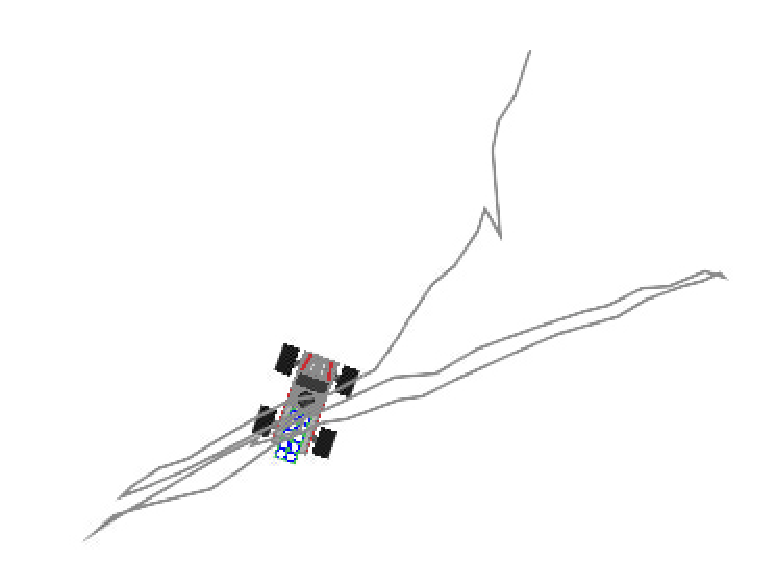
\includegraphics[width=0.4\linewidth]{resource/localization-simulation.pdf}
	\end{center}
	\caption{Results of the localization simulation}
	\label{fig:sim-loc-res}
\end{figure}

Figure~\ref{fig:sim-sys-res} shows the results of the small system simulation. We had KITT to drive to two waypoints and eventually stop. The simulation verifies this that KITT operated correctly.

\begin{figure}[H]
	\begin{center}
		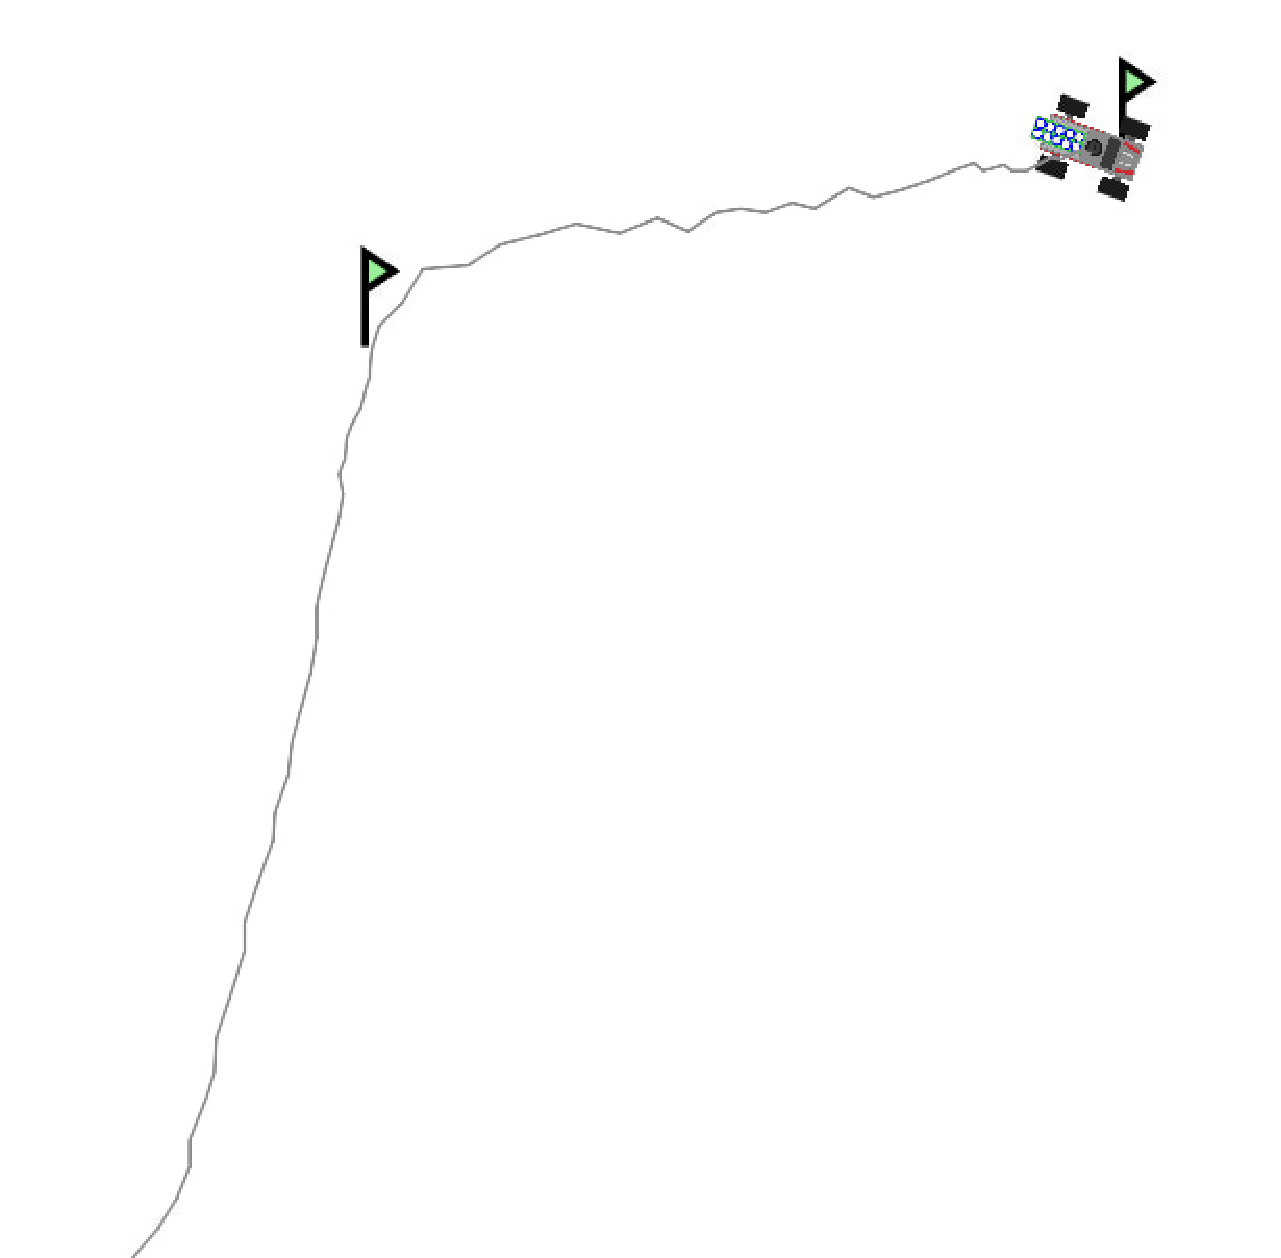
\includegraphics[width=0.7\linewidth]{resource/system-simulation.pdf}
	\end{center}
	\caption{Results of the small system simulation}
	\label{fig:sim-sys-res}
\end{figure}

\section{Conclusion}
The simulation results turned out to be as expected. This made us confident that our system had a good chance of working.

\end{document}